\section{Simulation Apps}

\subsection{Explanation of Building Bricks}

\subsubsection{Input: Parameter Sets}
\label{sec:parametersets}

Parameter sets are a hierarchical collection of parameters. Parameters can be of different type, see table \ref{tab:parameters} for a list.

A parameter set constitutes the full input data set for an analysis.

Beyond these primitive parameter types, there can be compounds, namely:
\begin{itemize}
\item \texttt{subset}

a subdirectory in a parameter set

\item \texttt{selectablesubset}

a \texttt{subset} that switches its content based on a \texttt{selection} parameter

\item \texttt{array}

an array of either a compound parameter or a primitve parameter
\end{itemize}

Throughout this manual and also e.g. in the command line parameters, the parameters are commonly specified in a file path-like format, where subsections are separated by slashes.
For example, the parameter \texttt{evaluateonly} in the subsection \texttt{run} is meant by the expression \texttt{run/evaluateonly}.

For arrays elements, the index of the element is inserted after the array parameter name. For example, the parameter \texttt{mesh/refinementZones/0/lx} refers to the parameter \texttt{lx} inside the first array element of the array of subsections \texttt{refinementZones} in the subsection \texttt{mesh}.

\begin{table}[h!]
\centering
\begin{tabular}{ll}
\hline
Type & Description \\
\hline\hline
\texttt{double} & a scalar floating point value\\
\texttt{int} & an integer value\\
\texttt{bool} & a boolean value\\
\texttt{vector} & a 3-tuple of doubles\\
\texttt{string} & a simple text\\
\texttt{selection} & a selection from a predefined set\\
\texttt{path} & a file path, relative to the input file\\
\texttt{matrix} & a matrix with arbitrary number of rows and cols\\
\texttt{doublerange} & an array of double values\\
\hline
\end{tabular}
\caption{Available primitive parameter types in a parameter set}
\label{tab:parameters}
\end{table}

\subsubsection{Output: Results Sets}

The output of an analysis is stored in a result set. 
It may contain elements like charts, images, tables, number etc.
A result set can be saved to a XML file and/or rendered into a PDF report.

\subsubsection{Analyses: the Simulation Procedure}

The procedure of a simulation is contained in a so-called analyses or workflow module.
You may think of it as an app for executing a certain type of simulation.
It is essentially a program.
Oftentimes, people create scripts or macros for speeding up their simulation workflows.
The InsightCAE workflow modules serve a similar purpose, though the intention is to fully cover the whole simulation including all pre and post processing steps.

There is a GUI available which provides an editor for the input parameter set (see section \ref{sec:workbench}).
The GUI is also capable of displaying a 3D preview of the involved geometry and other elements, which are displayable.
The analysis module is responsible of creating the 3D preview elements.
Creation of the preview is optional and not every analysis module produces a preview.

The GUI also includes a viewer for the result set. From that viewer, the reports may be exported.

InsightCAE holds a runtime-extensible list of available analyses.
This list can be extended at run time either by providing shared libraries containing more analysis modules or by python scripts.

The analyses can be programmed essentially in C++ or in Python.
InsightCAE is essentially written in C++. Python wrappers for the relevant functions and objects are created using SWIG. So the API can also be accessed from Python.

If a new analysis shall be created, this parameter editing and result viewing infrastructure is easily reusable:
\begin{itemize}
\item The new analysis module just needs to provide the parameter set layout by returning the default parameter set (a parameter set filled with suitable default values),
\item it has to provide a function for executing the analysis.
\item This function needs to return a result set.
\end{itemize}

The analysis modules may group themselves into categories. This is used in the initial analysis creation dialog in the GUI.

\paragraph{Python Script}

A python based analysis comprises a single dedicated python script file.
The InsightCAE functions are included by an initial statement like \verb!from Insight.toolkit import *!.

This script needs to define three standalone functions:
\begin{enumerate}
\item \verb!category()!

This functions returns a plain string with the category of the analysis. Multiple hierarchy levels are supported and have to be separated by slashes.

\item \verb!defaultParameters()!

This function shall return an object of type \texttt{ParameterSet}, containing the default values of all the needed parameters. The user cannot add or delete parameters, just modify their values. So this defines the layout.

\item \verb!executeAnalysis(parameters, workdir)!

This function finally runs the simulation.
It gets an object of type \verb!ParameterSet!, containing all the input parameters and the string \texttt{workdir}, which contains the execution directory.

\end{enumerate}

Upon loading, the InsightCAE base library searches in 
\begin{itemize}
\item \texttt{\$INSIGHT\_GLOBALSHAREDDIRS/python\_modules} and
\item \texttt{\$INSIGHT\_USERSHAREDDIRS/python\_modules}
\end{itemize}  for files named \texttt{*.py}. 
Each of these files will be loaded and their defined analyses will become available in the GUI and all other InsightCAE tools.


\paragraph{C++}

In C++, a new analysis is derived from the common base class \texttt{Analysis}.
The necessary functions have to be overridden.
The new analysis should be put into a dedicated shared library.

Upon loading, the InsightCAE base library searches in 
\begin{itemize}
\item \texttt{\$INSIGHT\_GLOBALSHAREDDIRS/modules.d} and
\item \texttt{\$INSIGHT\_USERSHAREDDIRS/modules.d}
\end{itemize}
for files named \texttt{*.module}. 
Each of these files has to contain a statement \verb!library <FILENAME>!, where FILENAME is the name of the shared library file. These libraries will all be loaded and their defined analyses will become available in the GUI and all other InsightCAE tools.

\subsection{Usage}

\subsubsection{GUI: workbench}
\label{sec:workbench}

The GUI for editing analysis parameters, run analyses and monitor their progress and to review the result sets is called \texttt{workbench}.

It can be started from the command line by executing
\begin{lstlisting}[language=bash]
$ workbench
\end{lstlisting}
or from the global application menu.

The workbench can open and handle multiple analyses at a time. For each analysis, a sub window is opened (analysis form).

An analysis can either be created from scratch (\seenameref{par:workbench:new_analysis}) or by opening an existing analysis input file (select \menu{Analysis>Open...} in the menu).

The analysis form has three tabs. From left to right: the input parameter edit tab, the progress display tab and the result viewer tab.

\paragraph{Editing the Input Parameters}
The parameter input tab is shown in figure \ref{fig:workbench_parameters}. On the left, there is a tree view showing all the available parameters of the analysis.
The font display style of the parameter entry denotes the importance of the parameter:
\begin{itemize}

\item highlighted yellow background: these parameters have no reasonable default values and need to be changed for every case. The displayed default values are only chosen to demonstrate some functional value, e.g. for speeds or rpms. But for parameters like file names, for  example, there is no reasonable default at all.

\item normal black text color: these parameters have reasonable default values, with which an analysis can be started. Though it is quite normal, that these parameters might need to be adapted from case to case.

\item dimmed gray text color: these parameters should normally be left at their default values. But it for rather rare special cases, it might become necessary to adapt them.
\end{itemize}

The parameters can be selected my mouse click and edited (\seenameref{par:workbench:change_parameter}).

Some analyses (this is optional) support a 3D preview of the configured case.
When an analysis is loaded, which supports 3D preview, a 3D view and a 3D element tree appears right of the parameter edit column.
All views in the Input tab are shown in a horizontal splitter and their width can be adapted by dragging the splitter handle between them. It is also possible to hide the 3D preview widgets by collapsing their width to zero using the splitter handle (This might also occur accidentally). The collapsing can be undone by locating the splitter handle of the collapsed widget and dragging it back to some non-zero width.
The layout of the splitter is saved on program exit and restored on the next start.

\paragraph{Saving Parameters}
\label{par:save_parameters}
Once all parameters are edited, the parameter set can be saved to a file.
Very often, external files are referenced from a parameter set.
Since it is also often necessary, to relocate parameter sets from one computer to another or between directories, InsightCAE parameter sets provide some special features which shall simplify relocation of parameter sets:
\begin{itemize}
\item file paths are always stored as relative paths inside the parameter set file.

Even if the workbench editor displays an absolute path, the paths are made relative to the saving location of the parameter set file. It is still possible to insert absolute paths into a parameter set file. But when it is loaded and saved again, these will be made relative.

If a parameter set is moved around together with the files it references, they will be found, as long as they remain in the same relative location, e.g. side by side with the parameter file or in a sub directory.

\item external files can be embedded into the parameter file.

This is the preferred option, when parameter files shall be moved across computers. Upon saving, the files will be base-64 encoded (not compressed) and stored in the XML file.
When the analysis is run, the files are extracted to a temporary location.
The extraction is aware of the case, that different files with the same name might exist in different directories and extracts them to different locations.
By default, the files are extracted to the system temporary location.
When the InsightCAE application, which triggered the extraction of the parameter, exits, the files are deleted again from the temporary location. Note that this might not be achieved, if the application crashes.

Packing of external files can be enabled by checking \menu{Parameters>Pack external files into parameter file} or by checking the appropriate option in the "Save Parameters" dialog.
Once, a parameter file was saved as packed or unpacked, the selection state is saved and used for all subsequent save operations.

\end{itemize}

\paragraph{Running the Analysis}
With a properly edited parameter set, the analysis run can be started.
This is achieved by clicking on the button "Run" on the right side or by selecting \menu{Actions>Run Analysis} in the menu.
This analysis form switches automatically to the "Run" tab (see figure \ref{fig:workbench_progress}).
In the lower half, the log message are displayed.
Sometimes, errors in an external program occur and are not correctly reported. 
It is therefore a good practice to watch the log messages for errors or warnings.

When the simulation solver runs, InsightCAE shows progress variables graphically.
The plots are shown above the log widget.
The number and meaning of the progress variables depend on the analysis conducted.

Especially for OpenFOAM-bases analyses, a number of quantities are extracted from solver output and forwarded to the GUI as progress variables:
\begin{itemize}
\item continuity errors
\item equation residuals
\item forces
\item moments
\item execution time (per timestep)
\end{itemize}

\paragraph{Cancel a Simulation}
To cancel a simulation run, click on the button "Kill" on the right side or by select \menu{Actions>Stop Analysis} in the menu.

\paragraph{Viewing the Results}
Once the simulation run is finished (that means that the solver has finished and that all post processing steps are done), a result set is created and loaded into the workbench.
It is displayed in the "output" tab (see figure \ref{fig:workbench_result}).
The result set can be rendered into a report (\seenameref{par:workbench:create_report}).


\paragraph{Rendering Results into a Report}\label{par:workbench:create_report}


\paragraph{Modifying a Parameter}\label{par:workbench:change_parameter}

\paragraph{Creating a New Analysis}\label{par:workbench:new_analysis}
A new analysis is created by selecting in the menu \menu{Analysis>New...}. Then a new dialog appears, in which the list of available analyses is displayed (figure \ref{fig:workbench_new_analysis}).
The required analysis should be selected and confirmed by clicking "Ok".

\begin{figure}[tb]
\centering
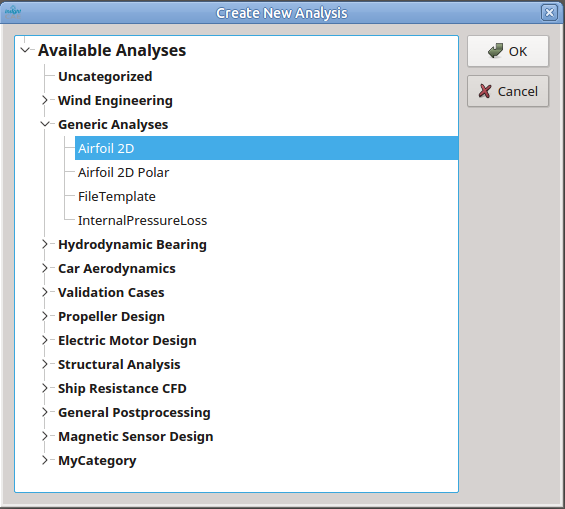
\includegraphics[width=0.5\linewidth]{figs/workbench/workbench_new_analysis}
\caption{Dialog for selection of the type of a new analysis}
\label{fig:workbench_new_analysis}
\end{figure}



\begin{figure}[tb]
\centering
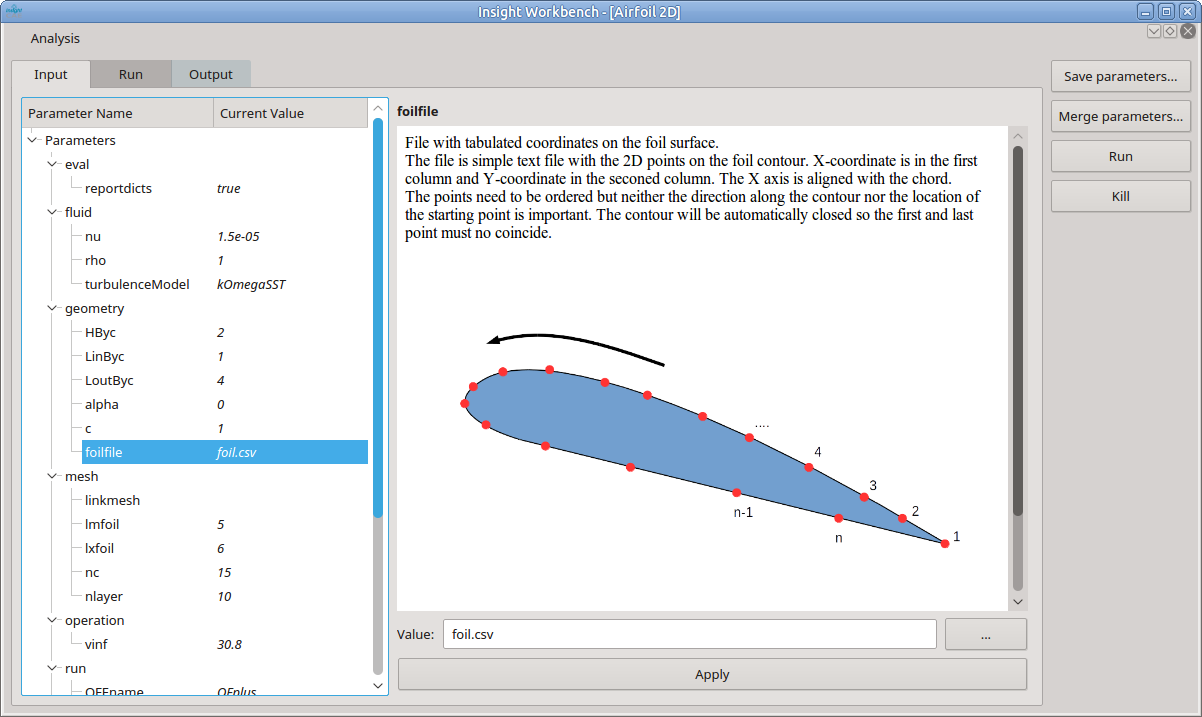
\includegraphics[width=\linewidth]{figs/workbench/workbench_airfoil_parameters}
\caption{Parameter editing tab of the workbench}
\label{fig:workbench_parameters}
\end{figure}

\begin{figure}[tb]
\centering
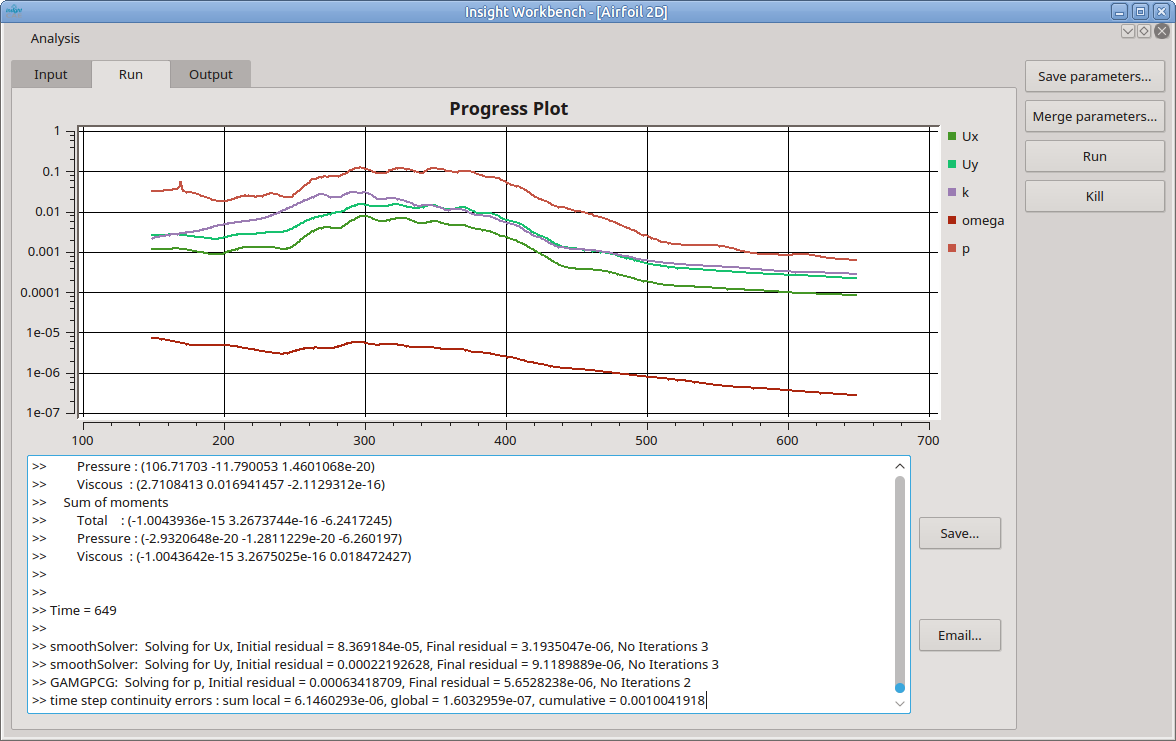
\includegraphics[width=\linewidth]{figs/workbench/workbench_airfoil_run}
\caption{Solution progress tab of the workbench}
\label{fig:workbench_progress}
\end{figure}

\begin{figure}[tb]
\centering
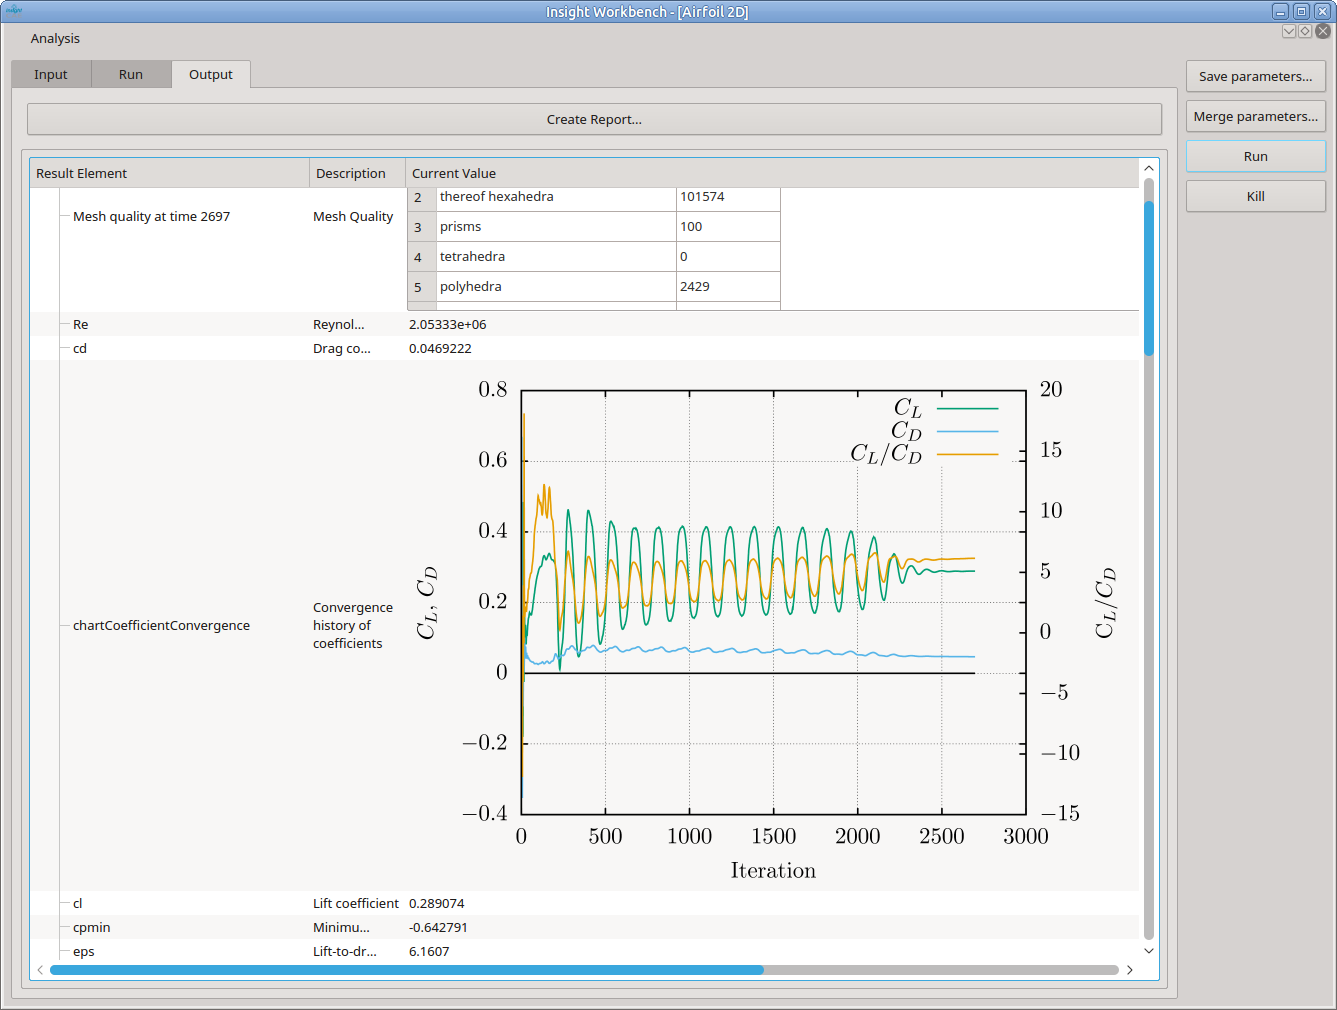
\includegraphics[width=\linewidth]{figs/workbench/workbench_airfoil_result}
\caption{Result explorer tab of the workbench}
\label{fig:workbench_result}
\end{figure}

\subsubsection{Special Features for OpenFOAM-based Simulation Apps}

Simulation apps which are based on an OpenFOAM simulation provide some special features and also some implicit behavior and conventions which is documented in this section.

\paragraph{Restart Behavior}
OpenFOAM-based simulations often run for a long time. 
It frequently appears that the simulation procedure is interrupted, either accidentally or intentional, and needs to be restarted.

There is no explicit function for a restart.
It happens implicitly, when the analysis is re-launched in an existing working directory and some preconditions are met.

Depending on the state of the data, the behavior will be as follows:
\begin{itemize}

\item if a mesh exists (in folder "constant/polyMesh/") and a time directory exists (e.g. "0/"): it is assumed that the case is ready for execution and the solver will be restarted,

\item if only the mesh exists ("constant/polyMesh/") and no time directory: mesh creation will be skipped. But all the dictionaries in \texttt{constant/} and \texttt{system/} and field files in the initial time directory will be recreated.

\end{itemize}

Depending on where the interruption happened, the state might be inconsistent and invalid behavior might result.
For example:
\begin{itemize}
\item the interruption appeared within a meshing procedure which includes intermediate meshes $\Rightarrow$ a mesh will be present but invalid
\item the interruption appeared during the field initialization $\Rightarrow$ a time directory is present but the fields are invalid,
\item the interruption appeared during writing of a time directory $\Rightarrow$ a time directory is present but invalid and the solver restart will fail.
\end{itemize}

If you are unsure about the validity of the case data, please consider to clean the case directory first and restart everything from the beginning (see \ref{sec:cleancase}).

\paragraph{Cleaning the Case Directory}
\label{sec:cleancase}

When an OpenFOAM-based simulation run was performed, a number of directories and files are created in the working directory.
If another run shall be performed and no restart is desired, then these directories and files need to be removed first.
For this task, there is the standalone tool \texttt{isofCleanCase}, see section \ref{sec:isofcleancase}.

This tool can be launched in the selected workspace directory from within the GUI via the button "Clean" on the right side of the analysis form. Please see section \ref{sec:isofcleancase} for details on the usage.

In some OpenFOAM-based simulation apps, auxiliary OpenFOAM case are created in subdirectories of the workspace directory.
Currently, these can only be deleted or cleaned manually via a file manager and the command line tool \texttt{isofCleanCase}.



\paragraph{Performing only the Evaluation without Running the Solver}
\label{sec:evaluateonly_workbench}

This is needed, if the solver was manually restarted, e.g. after manual changes of the numerical settings became necessary due to stability problems and ran until completion in the case directory which the corresponding InsightCAE simulation app has created.

It is then possible to execute only the evaluation part of the simulation app alone.
This will not do any modifications to the simulation setup and it will not start any solver.
To do this, the following is needed:
\begin{enumerate}
\item in the parameter set, set the switch \texttt{run/evaluateonly} to \texttt{true},
\item set the working directory to the existing case directory, where the case was created (this will be done automatically, if an existing input file was opened),
\item then start the simulation by clicking the "Run" button.
\end{enumerate}

Please note, that all parameters in the input file are assumed to match the simulation setup. 
No checks are done and there is no possibility for the Simulation app to restore them from an existing simulation folder.
Thus it is up to the user to ensure validity.

\paragraph{Launching Graphical Postprocessor ParaView}

To inspect the results of a OpenFOAM simulation beyond the figure which the InsightCAE simulation extracts automatically from the simulation case, the independent graphical postprocessor Paraview can be used.

It can be launched from the command line using a script as explained in \ref{par:isPVpy}.

Alternatively, this can be done also from the workbench. On the right border of the analysis form, there is a button labelled "ParaView".
For OpenFOAM-based simulation apps, this is enabled.
Once it is pressed, Paraview will be launched in the selected working directory. 
If a local run is configured, it will just read the case from the selected working directory.
If a remote run is selected, a client-server pair will be launched and the connection to the remote side is set up via SSH tunnels.



\subsubsection{Console on Headless Computers: analyze}\label{sec:analyze}

It is possible to launch an analysis from an existing input file (*.ist) without the graphical user interface in a batch mode.
This is useful to integrate InsightCAE into workflows with other third-party software.
The input file can be saved from the workbench (see \ref{par:save_parameters}) or created by a script or with any text editor.

To launch a simulation in batch mode, the executable \texttt{analyze} is available.
It can be launched like this from the command line:

\begin{lstlisting}[language=bash]
$ analyze inputfile.ist
\end{lstlisting}

The executable understands additional options.
These are explanined in the following paragraphs.

\paragraph{Changing parameters}
The values of parameters in the input file can be overridden from the command line by specifying an arbitrary number of the following parameters:
\begin{itemize}
\item \texttt{-b [ --bool ] arg}\\ boolean variable assignment
\item \texttt{-l [ --selection ] arg }\\selection variable assignment
\item \texttt{-s [ --string ] arg}\\string variable assignment
\item \texttt{-p [ --path ] arg}\\path variable assignment
\item \texttt{-d [ --double ] arg}\\double variable assignment
\item \texttt{-v [ --vector ] arg}\\vector variable assignment
\item \texttt{-i [ --int ] arg}\\integer variable assignment
\end{itemize}

The argument \texttt{arg} for all these options has the form:
\texttt{path:value}.
The path is the file path-like specification of the parameter (see \ref{sec:parametersets}) and the value is appended to the name, separated by a colon.
If any spaces are inside the value, e.g. when strings or path names are to be specified, then the entire \texttt{arg} should be set in qoutes at the command line. For example:
\begin{lstlisting}[language=bash]
$ analyze --path "run/mapFrom:/a/path/with spaces" inputfile.ist
\end{lstlisting}

\paragraph{General Behaviour}

The simulation working directory can be set explicitly by the parameter \texttt{--workdir} (short \texttt{-w}). 
The default is to use the current directory as the working directory.

The finally applied input parameter set is optionally saved to a file, when the file is specified with the parameter \texttt{--savecfg} (short \texttt{-c}).

\subsection{Available Simulation Workflows}

\subsubsection{Numerical Wind Tunnel}

\subsubsection{Internal Pressure Loss}
